% Figure s05f05_kitaev (Session 5): the Kitaev chain, which Majoranas pair with which.
% The image is rendered by figures/blender/s05f05_kitaev.py; the coordinates of the labels come from
% figures/blender/out/s05f05_kitaev_anchors.tex. Build with figures/blender/build_figure.sh s05f05_kitaev.
\documentclass[11pt,tikz,border=0pt]{standalone}
\usepackage[T1]{fontenc}
\usepackage{amsmath,amssymb,graphicx,bm}
\usepackage{xcolor}
\usetikzlibrary{arrows.meta,calc}
% The three label colors of the figures, with the same values as in src/figures_preamble.tex.
\definecolor{aqmaccent}{RGB}{31,78,121}
\definecolor{aqmbroken}{RGB}{168,42,34}
\definecolor{aqmmuted}{RGB}{125,125,125}

\newlength{\figw}\setlength{\figw}{15.6cm}   % the text width of the notes (A4, 2.7 cm margins)

\begin{document}
\begin{tikzpicture}[lbl/.style={font=\small, inner sep=1.5pt}, pnl/.style={font=\small\bfseries, inner sep=1.5pt}]
  \node[anchor=south west, inner sep=0pt] at (0,0)
    {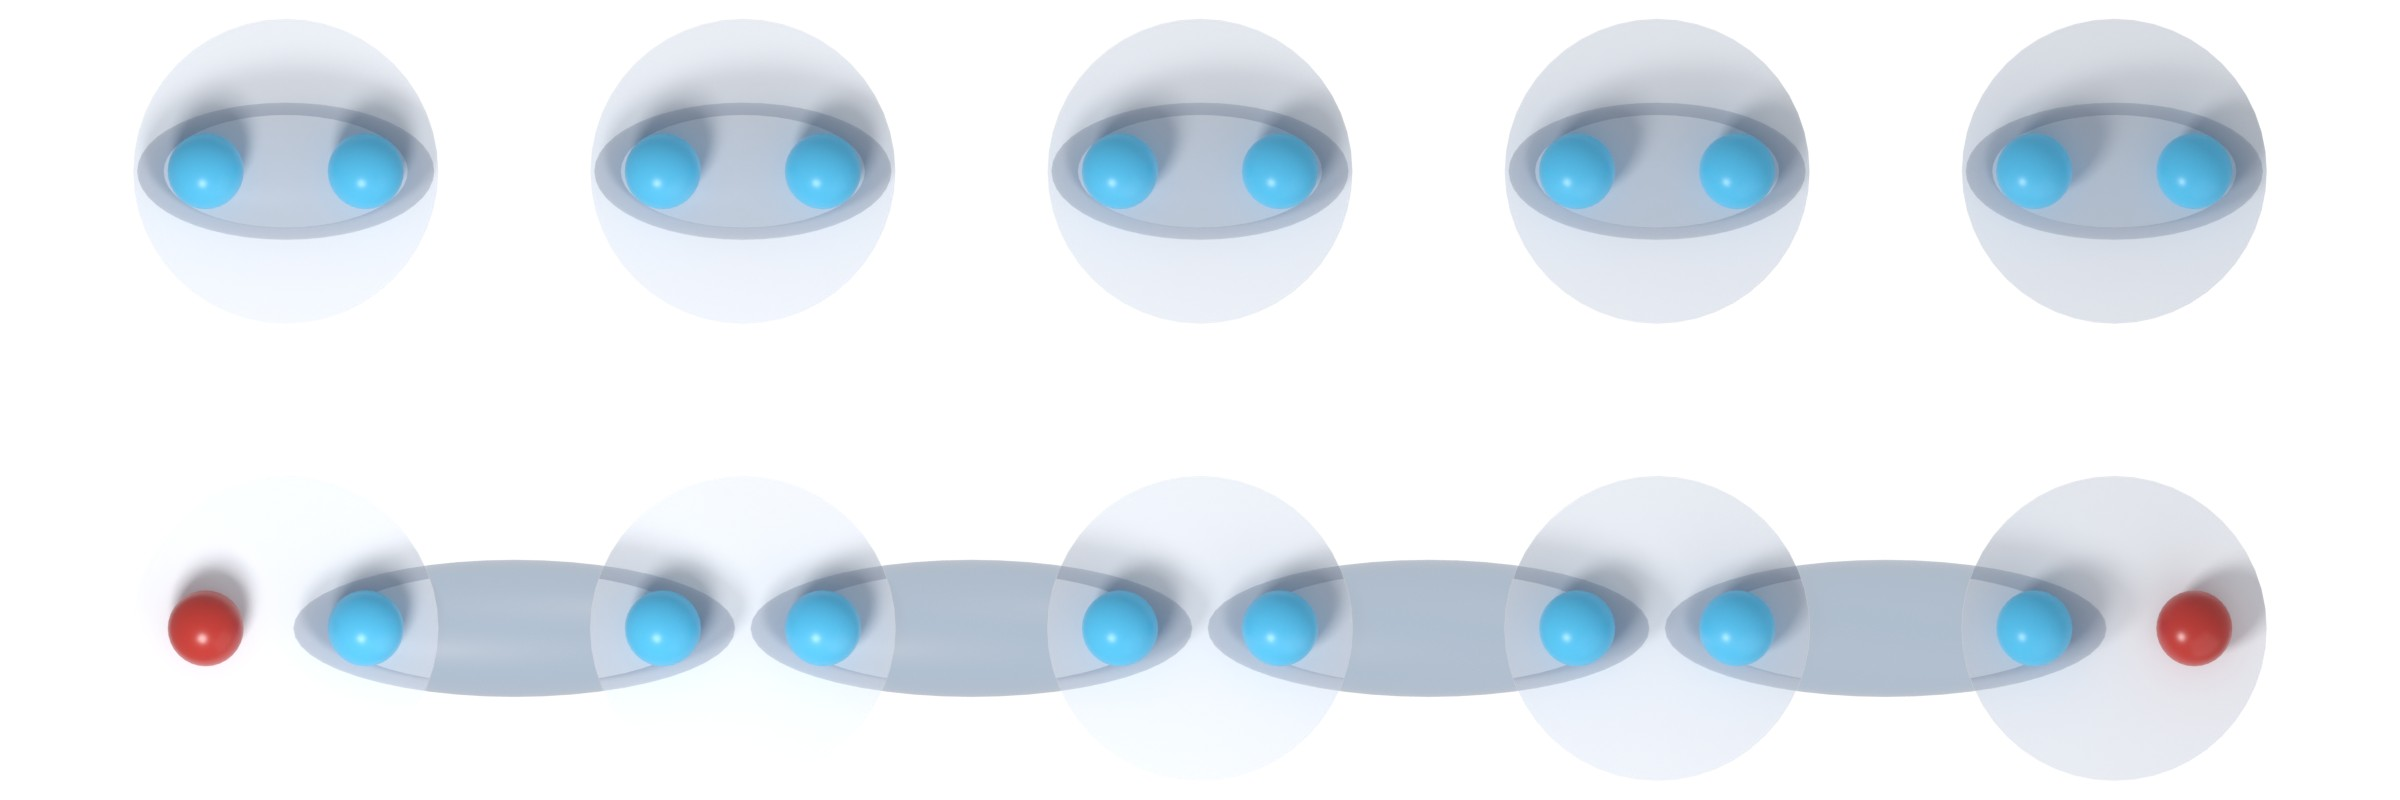
\includegraphics[width=\figw]{../blender/out/s05f05_kitaev.jpg}};
  %% written by figlib.py; x and y in units of the image width
\coordinate (tg1) at (0.0857\figw,0.2382\figw);
\coordinate (tg2) at (0.1524\figw,0.2382\figw);
\coordinate (tg3) at (0.2762\figw,0.2382\figw);
\coordinate (tg4) at (0.3429\figw,0.2382\figw);
\coordinate (tg5) at (0.4667\figw,0.2382\figw);
\coordinate (tg6) at (0.5333\figw,0.2382\figw);
\coordinate (tg7) at (0.6571\figw,0.2382\figw);
\coordinate (tg8) at (0.7238\figw,0.2382\figw);
\coordinate (tg9) at (0.8476\figw,0.2382\figw);
\coordinate (tg10) at (0.9143\figw,0.2382\figw);
\coordinate (tpanel) at (0.0357\figw,0.3374\figw);
\coordinate (bg1) at (0.0857\figw,0.0477\figw);
\coordinate (bg2) at (0.1524\figw,0.0477\figw);
\coordinate (bg3) at (0.2762\figw,0.0477\figw);
\coordinate (bg4) at (0.3429\figw,0.0477\figw);
\coordinate (bg5) at (0.4667\figw,0.0477\figw);
\coordinate (bg6) at (0.5333\figw,0.0477\figw);
\coordinate (bg7) at (0.6571\figw,0.0477\figw);
\coordinate (bg8) at (0.7238\figw,0.0477\figw);
\coordinate (bg9) at (0.8476\figw,0.0477\figw);
\coordinate (bg10) at (0.9143\figw,0.0477\figw);
\coordinate (bpanel) at (0.0357\figw,0.1469\figw);

  \node[lbl, anchor=south west] at (tpanel) {\textbf{trivial}, binding inside each site};
  \node[lbl, anchor=south west] at (bpanel) {\textbf{topological}, binding between sites};
  \node[lbl, anchor=north] at (tg1) {$\gamma_1$};
  \node[lbl, anchor=north, text=aqmbroken] at (bg1) {$\gamma_1$};
  \foreach \p in {t,b} {
    \node[lbl, anchor=north] at (\p g2) {$\gamma_2$};
    \node[lbl, anchor=north] at (\p g3) {$\gamma_3$};
    \node[lbl, anchor=north] at (\p g9) {$\gamma_9$};
  }
  \node[lbl, anchor=north] at (tg10) {$\gamma_{10}$};
  \node[lbl, anchor=north, text=aqmbroken] at (bg10) {$\gamma_{10}$};
\end{tikzpicture}
\end{document}
